\documentclass[10pt,a4paper,twoside]{article}
\usepackage[english]{babel}
%laad de pakketten nodig om wiskunde weer te geven :
\usepackage{amsmath,amssymb,amsfonts,textcomp}
%laad de pakketten voor figuren :
\usepackage{graphicx}
\usepackage{float,flafter}
\usepackage{hyperref}
\usepackage{inputenc}
\usepackage{minted}
\usepackage{subcaption}

\setlength\paperwidth{20.999cm}\setlength\paperheight{29.699cm}\setlength\voffset{-1in}\setlength\hoffset{-1in}\setlength\topmargin{1.499cm}\setlength\headheight{12pt}\setlength\headsep{0cm}\setlength\footskip{1.131cm}\setlength\textheight{25cm}\setlength\oddsidemargin{2.499cm}\setlength\textwidth{15.999cm}

\newcommand{\sweepsize}{0.26}

\begin{document}
\begin{center}
\hrule

\vspace{.4cm}
{\bf {\Huge Computer Vision} \\ {\huge Lab Assigment Report} \\ {\Large Condensation Tracker}}
\vspace{.2cm}
\end{center}
{\bf Tuan Mate Nguyen}  (tunguyen@student.ethz.ch)
\hrule


\section{Implementation}
\subsection{Color histogram}
For the histogram only pixels in the bounding box of the ROI are considered. This sub-array is then flattened as
required by np.histogramdd(), which is a function for creating multidimensional
histograms. As there are 3 color channels and $hist\_bin$ number of bins for each
color dimension, the resulting histogram will have a size of $hist\_bin^3$.

\begin{minted}[mathescape,
    linenos,
    numbersep=5pt,
    gobble=2,
    frame=lines,
    framesep=2mm,
    firstnumber=4]{csharp}
    roi = frame[ymin:ymax, xmin:xmax]
    flat_roi = roi.reshape(-1, 3)
    hist, _ = np.histogramdd(flat_roi, hist_bin, [[0, 255]]*3, density=False)
\end{minted}

The density parameter is set to false in order to obtain the number of samples in
each bin. Then the bins are explicitly normalized by dividing the total number of
samples.

\subsection{$A$ matrix}
In case of no motion the state vector consists of only two elements,
corresponding to the $x$ and $y$ coordinates of the object. Since the prediction
model assumes no motion, the coordinates remain the same after applying the
deterministic part of the system transition function. Thus, the $A$ matrix will
just be the identity matrix

\[ A_{no motion} =
\begin{bmatrix}
    1 & 0 \\
    0 & 1 
\end{bmatrix}
\]

As for the constant velocity model, the state vector has 4 elements, the two
spatial coordinates and the velocities in the $x$ and $y$
directions. For the new coordinates - ignoring dimensions - the deterministic
transition function can be written as

\[ x_t = x_{t-1} + v_{x_{t-1}} \]
\[ y_t = y_{t-1} + v_{y_{t-1}} \].

The velocities remain constant so in the bottom block the diagonal elements will
be 1 and everything else 0.

\[ A_{const. velocity} =
\begin{bmatrix}
    1 & 0 & 1 & 0 \\
    0 & 1 & 0 & 1 \\ 
    0 & 0 & 1 & 0 \\ 
    0 & 0 & 0 & 1 \\ 
\end{bmatrix}
\]

\subsection{Propagation}

The system then can be propagated by computing
\[
s_t^{(n)} = A{s^{'}}_{t-1}^{(n)} + w_{t-1}
\]
for every particle. Here $w_{t-1}^{(n)}$ is of shape (2,2) for the no motion
model (coordinate noise only) and (4,2) for the constant velocity model (both
coordinate and velocity perturbations). Its values are obtained by sampling from
a normal distribution with 0 mean and $\sigma_{pos}$ and $\sigma_{vel}$
standard deviation for the coordinates and velocities, respectively.

This operation could potentially result in particles located outside of the
frame. The chosen method to handle this is to clamp the updated coordinates so
that they remain inside the frame.

\begin{minted}[mathescape,
    linenos,
    numbersep=5pt,
    gobble=2,
    frame=lines,
    framesep=2mm,
    firstnumber=21]{csharp}
    xs = new_particles[:,0] < 0
    ys = new_particles[:,1] < 0
    new_particles[xs, 0] = 0
    new_particles[ys, 1] = 0
    
    xs = new_particles[:,0] >= frame_width
    ys = new_particles[:,1] >= frame_height
    new_particles[xs, 0] = frame_width-1
    new_particles[ys, 1] = frame_height-1
\end{minted}


\subsection{Observation}

In the observation step for each particle, first the bounding box needs to be
determined. The corner points can then be fed to the previously described color
histogram computing function. It is worth mentioning that in my implementation
objects on the image border will have a smaller bounding box than the original.
This could lead to slightly different color histogram as only a portion of the
object's colors are taken into account.  However, since the output doesn't
matter once the object leaves the frame, this is acceptable. Then the current
color histogram can be compared to the original one by taking their $\chi^2$
distance. The weight will be the Gaussian of this distance, parameterized by 0
mean and $\sigma_{observe}$ standard deviation. 

\begin{minted}[mathescape,
    linenos,
    numbersep=5pt,
    gobble=2,
    frame=lines,
    framesep=2mm,
    firstnumber=13]{csharp}
    # for every particle
    xmin = min(max(0, round(p[0]-half_w)), frame_width-1)
    ymin = min(max(0, round(p[1]-half_h)), frame_height-1)
    xmax = min(max(0, round(p[0]+half_w)), frame_width)
    ymax = min(max(0, round(p[1]+half_h)), frame_height)

    current_hist = color_histogram(xmin, ymin, xmax, ymax, frame, hist_bin)
    chi_dist = chi2_cost(hist, current_hist)
    weight = 1./(np.sqrt(2 * np.pi) * sigma_observe) * 
             np.exp(-1*(chi_dist * chi_dist) / (2 * sigma_observe * sigma_observe))
\end{minted}

Since the weights are used in a probabilistic context in the sampling step, we
need to normalize them so that their sum is 1.

\subsection{Estimation}

The mean state implementation is straight-forward, just taking a weighted sum of all particle states using their weights.
\begin{minted}[mathescape,
    linenos,
    numbersep=5pt,
    gobble=2,
    frame=lines,
    framesep=2mm,
    firstnumber=4]{csharp}
    mean_state = np.sum(particles * particles_w, axis=0)
\end{minted}

\subsection{Resampling}

For resampling first the particles and their current weights are paired so that
the resampled particles' weights are known.
\begin{minted}[mathescape,
    linenos,
    numbersep=5pt,
    gobble=2,
    frame=lines,
    framesep=2mm,
    firstnumber=4]{csharp}
    p = np.concatenate((particles, particles_w), axis=1)
\end{minted}
The sampling with replacement is convenient with numpy's random.Generator.choice() method, where the
chosen random number generator is the default one. The result is separated back into to particles
and their weights, and the weights are normalized (their sum is 1).
\begin{minted}[mathescape,
    linenos,
    numbersep=5pt,
    gobble=2,
    frame=lines,
    framesep=2mm,
    firstnumber=6]{csharp}
    # rng is a global variable: np.random.default_rng()
    p_new = rng.choice(p, size=particles.shape[0], replace=True, p=particles_w.reshape(-1), axis=0)
    n_dim = particles.shape[1]
    sampled_particles = p_new[:, :n_dim]
    sampled_weights = p_new[:, n_dim]
    sampled_weights = sampled_weights / np.sum(sampled_weights)
\end{minted}

\section{Experiments}

For the experiments in this section instead of selecting the starting bounding boxes
manually every time, I hardcoded them to the following values to make comparison
between different parameters more accurate.
\begin{table}[h!]
\begin{center}
    \begin{tabular}{ c c c } 
     \hline
     Video & Top left & Bottom right\\
     \hline
     \hline
     1 & (128, 99)& (142, 111)\\ 
     \hline
     2 & (7, 70)&(20, 87)\\
     \hline
     3 & (24, 87)&(31, 95)\\
     \hline
    \end{tabular}
\end{center}
\end{table}    

 %=====================================================================================



\subsection{Video 1}

For the no motion model even the default values worked fairly well. Small
$\sigma_{position}$ version was a bit noisier. 

Tested number of particles were 30, 100, 200 and 300, resulting in similar quality. In case of this simpler video it
didn't really matter but in later, more complex videos using more
points proved to be more robust. Consequently the number of points were set to 300.

Different bin numbers (4, 16, 32) also yielded similar results, however, at 64
the tracked trajectory became too noisy as the histograms of sampled particles
near the object didn't match well enough due to the higher resolution of bins.

Updating the appearance model helped, after setting the $\alpha$ value higher
than $0.5-0.7$ results were more accurate. Without updating the center of the
hand was missed (mean was located slightly below, where the arm was similarly
dark as original hand).
%appearance model: 0.1 false track, 0.3 < 0.5~0.7~0.9~1.0 best so far
%with 0 it always stays bit below hand -> darker image originally; with update its more the center

\begin{figure}[h]
    \centering
    \begin{subfigure}{\sweepsize\textwidth}
    \includegraphics[width=0.9\linewidth]{1/1_hb32_np300_mm0_am0.7_sp5_sv2_11.png} 
    \end{subfigure}
    \begin{subfigure}{\sweepsize\textwidth}
    \includegraphics[width=0.9\linewidth]{1/1_hb32_np300_mm0_am0.7_sp5_sv2_17.png} 
    \end{subfigure}
    \begin{subfigure}{\sweepsize\textwidth}
    \includegraphics[width=0.9\linewidth]{1/1_hb32_np300_mm0_am0.7_sp5_sv2_23.png} 
    \end{subfigure}
    \begin{subfigure}{\sweepsize\textwidth}
    \includegraphics[width=0.9\linewidth]{1/1_hb32_np300_mm0_am0.7_sp5_sv2_29.png} 
    \end{subfigure}
    \begin{subfigure}{\sweepsize\textwidth}
    \includegraphics[width=0.9\linewidth]{1/1_hb32_np300_mm0_am0.7_sp5_sv2_35.png} 
    \end{subfigure}
    \begin{subfigure}{\sweepsize\textwidth}
    \includegraphics[width=0.9\linewidth]{1/1_hb32_np300_mm0_am0.7_sp5_sv2_41.png} 
    \end{subfigure}
    \caption{Result for no motion model, with $\sigma_{pos}=5$, $\alpha=0.7$, $n_{points}=300$ and $hist\_bins=32$}
\end{figure}

The constant velocity model didn't work as well as the no motion model. This is
not surprising, as the motion was not constant but had sudden direction changes.
To handle these changes in velocity, $\sigma_{velocity}$ would need
to be big enough (comparable with initial velocity) so velocity could follow the
change but that would lead to spatially sparser sampling, making the system less stable. A
solution could be to use more points, where computing power could be a limiting factor.
%1_hb32_np300_mm1_am0.7_sp1_sv1_41

\begin{figure}[h]
    \centering
    \begin{subfigure}{\sweepsize\textwidth}
    \includegraphics[width=0.9\linewidth]{1/1_hb32_np300_mm1_am0.7_sp1_sv1_11.png} 
    \end{subfigure}
    \begin{subfigure}{\sweepsize\textwidth}
    \includegraphics[width=0.9\linewidth]{1/1_hb32_np300_mm1_am0.7_sp1_sv1_17.png} 
    \end{subfigure}
    \begin{subfigure}{\sweepsize\textwidth}
    \includegraphics[width=0.9\linewidth]{1/1_hb32_np300_mm1_am0.7_sp1_sv1_23.png} 
    \end{subfigure}
    \begin{subfigure}{\sweepsize\textwidth}
    \includegraphics[width=0.9\linewidth]{1/1_hb32_np300_mm1_am0.7_sp1_sv1_29.png} 
    \end{subfigure}
    \begin{subfigure}{\sweepsize\textwidth}
    \includegraphics[width=0.9\linewidth]{1/1_hb32_np300_mm1_am0.7_sp1_sv1_35.png} 
    \end{subfigure}
    \begin{subfigure}{\sweepsize\textwidth}
    \includegraphics[width=0.9\linewidth]{1/1_hb32_np300_mm1_am0.7_sp1_sv1_41.png} 
    \end{subfigure}
    \caption{Result for constant velocity model, with $\sigma_{pos}=1$,
    $\sigma_{velocity}=1$, $v_{initial}=(0, -4)$, $\alpha=0.7$, $n_{points}=300$
    and $hist\_bins=32$. Tracking is lost if sudden change in velocity occurs
    (sharp turn).}
\end{figure}

In general sudden movements are better modeled assuming no motion and just using
bigger standard deviation. In this case positions are independently generated for
every frame but for the constant velocity model the previous velocity vector
influences new coordinates, adding some inertia to the system.

\subsection{Video 2}

Using the best models from Video 1 don't work, the appearance update
prevents it. Reducing alpha to 0.1 helps, but still, the object is occluded for too
long. During this time the appearance model is altered to an extent that even
after the object reappears, its histogram doesn't match with the updated one.
Even if the constant velocity model was used, it doesn't work. Hence $\alpha$
was set to 0.

\begin{figure}[h]
    \centering
    \begin{subfigure}{\sweepsize\textwidth}
    \includegraphics[width=0.9\linewidth]{2/2_hb32_np300_mm0_am0.7_sp5_sv1_4.png} 
    \end{subfigure}
    \begin{subfigure}{\sweepsize\textwidth}
    \includegraphics[width=0.9\linewidth]{2/2_hb32_np300_mm0_am0.7_sp5_sv1_11.png} 
    \end{subfigure}
    \begin{subfigure}{\sweepsize\textwidth}
    \includegraphics[width=0.9\linewidth]{2/2_hb32_np300_mm0_am0.7_sp5_sv1_17.png} 
    \end{subfigure}
    \begin{subfigure}{\sweepsize\textwidth}
    \includegraphics[width=0.9\linewidth]{2/2_hb32_np300_mm0_am0.7_sp5_sv1_23.png} 
    \end{subfigure}
    \begin{subfigure}{\sweepsize\textwidth}
    \includegraphics[width=0.9\linewidth]{2/2_hb32_np300_mm0_am0.7_sp5_sv1_29.png} 
    \end{subfigure}
    \begin{subfigure}{\sweepsize\textwidth}
    \includegraphics[width=0.9\linewidth]{2/2_hb32_np300_mm0_am0.7_sp5_sv1_35.png} 
    \end{subfigure}
    \caption{Result for no motion model, with $\sigma_{pos}=5$, $\alpha=0.7$, $n_{points}=300$
    and $hist\_bins=32$. Appearance is changed too much, so original object is quickly lost.}
\end{figure}

\begin{figure}[h]
    \centering
    \begin{subfigure}{\sweepsize\textwidth}
    \includegraphics[width=0.9\linewidth]{2/2_hb32_np300_mm0_am0.1_sp5_sv1_4.png} 
    \end{subfigure}
    \begin{subfigure}{\sweepsize\textwidth}
    \includegraphics[width=0.9\linewidth]{2/2_hb32_np300_mm0_am0.1_sp5_sv1_11.png} 
    \end{subfigure}
    \begin{subfigure}{\sweepsize\textwidth}
    \includegraphics[width=0.9\linewidth]{2/2_hb32_np300_mm0_am0.1_sp5_sv1_17.png} 
    \end{subfigure}
    \begin{subfigure}{\sweepsize\textwidth}
    \includegraphics[width=0.9\linewidth]{2/2_hb32_np300_mm0_am0.1_sp5_sv1_23.png} 
    \end{subfigure}
    \begin{subfigure}{\sweepsize\textwidth}
    \includegraphics[width=0.9\linewidth]{2/2_hb32_np300_mm0_am0.1_sp5_sv1_29.png} 
    \end{subfigure}
    \begin{subfigure}{\sweepsize\textwidth}
    \includegraphics[width=0.9\linewidth]{2/2_hb32_np300_mm0_am0.1_sp5_sv1_35.png} 
    \end{subfigure}
    \caption{If $\alpha$ is reduced to 0.1, it works better, but the object is
    occluded for too long. With the mean state getting stuck  the appearance
    model is again changed too much, and the object is lost.}
\end{figure}
%solutions:
%don't update so much alpha=0.1 still doesn't work but almost, 0.0 works but gets confused at the end
%as the object is occluded by at least 50\% for several frames, alpha could significantly reduce the performance
%so lets fix alpha=0

Another potential issue with this setup is if $\sigma_{pos}$ is too small,
meaning that no points are sampled on the other side of the occluder, then the object
will not be picked up by the tracker after becoming visible again.

To make sure that the mean state doesn't get stuck after the object disappears, the
constant velocity model could be used. This is sensible as the movement of the
object is fairly constant. Thus if the initial velocity is set correctly, the
sampled particles' position will be shifted roughly by that amount and the
system becomes more robust against temporary occlusions (again, assuming
constant movement). Usage of smaller position noise will be tolerated as the "velocity
inertia" will keep the mean state moving across occluded regions.

%2_hb32_np300_mm1_am0.0_sp10_sv0_4
\begin{figure}[h]
    \centering
    \begin{subfigure}{\sweepsize\textwidth}
    \includegraphics[width=0.9\linewidth]{2/2_hb32_np300_mm1_am0.0_sp10_sv1_4.png} 
    \end{subfigure}
    \begin{subfigure}{\sweepsize\textwidth}
    \includegraphics[width=0.9\linewidth]{2/2_hb32_np300_mm1_am0.0_sp10_sv1_11.png} 
    \end{subfigure}
    \begin{subfigure}{\sweepsize\textwidth}
    \includegraphics[width=0.9\linewidth]{2/2_hb32_np300_mm1_am0.0_sp10_sv1_17.png} 
    \end{subfigure}
    \begin{subfigure}{\sweepsize\textwidth}
    \includegraphics[width=0.9\linewidth]{2/2_hb32_np300_mm1_am0.0_sp10_sv1_23.png} 
    \end{subfigure}
    \begin{subfigure}{\sweepsize\textwidth}
    \includegraphics[width=0.9\linewidth]{2/2_hb32_np300_mm1_am0.0_sp10_sv1_29.png} 
    \end{subfigure}
    \begin{subfigure}{\sweepsize\textwidth}
    \includegraphics[width=0.9\linewidth]{2/2_hb32_np300_mm1_am0.0_sp10_sv1_35.png} 
    \end{subfigure}
    \caption{Constant velocity model, with $\sigma_{pos}=10$, $\sigma_{velocity}=0$, $v=(3,0)$, $\alpha=0.0$, $n_{points}=300$
    and $hist\_bins=32$. Assuming constant velocity in the $x$ direction, and
    having larger $\sigma_{pos}$ to detect displacement in the $y$ direction
    works until the last section, where the hand starts moving faster, breaking
    the constand $v_x$ condition. Also there's some inaccuracy in front of the
    dark picture, where the histogram has higher dark pixel counts and the
    lighter colored wall could look more similar.}
\end{figure}

%Let's change system model!
%Constant velocity model's effect:
%More robust agains temporary occlusion: on average, as the constant velocity is
%kept (if tuned well in the beginning), the position distribution will be shifted
%by the constant velocity FOR EVERY FRAME. so eventhough the std.dev of position
%noise is not big enough tracking is not lost
%RESULT: pass occlusion

The effect of system noise if using smaller velocity noise means that only constant motion along a straight
line is expected. If there's some change in motion, however, then the position
noise needs to be bigger otherwise tracking won't be able to adapt to the actual motion as not enough points will be sampled near the object.

Using larger velocity noise could make the distance of the sampled points from
the object to quickly increase and make it difficult for tracking to find its
way back causing significant trajectory deviation. Actually it shouldn't be used, as the
original assumption was that the motion is constant, meaning the noise should be
small.

The effect of using bigger measurement noise would mean that we sample from particles with closer and closer to uniform distribution regardless of their resemblance to the object.
In a certain range it works - the measurement will be able to better distinct histograms as points close enough to the object will still have
relatively high weight compared to more distant ones. If the noise is too small, then the histogram corrsponding to perfectly matching position
would have much higher weight but sampling will always be random and probably this position will be missed so tracking will be
lost. Weights of more distant and closer particles will be equally small and the
sampling will again be approximately be uniform.

%measurement: determine velocity by measurement!
%????too small pos noise: in case of no motion tracking is blocked by the occlusion. Sensible, we're confident that 
%other:
%tracking for different alpha values if pos noise is 0, vel noise is 0.5, v =3,0.2
% - 0.3 doesn't work, 0.2 works

 %=====================================================================================

\subsection{Video 3}
In this case the appearance doesn't need to be updated because there's a big
contrast between the ball and the background and there's no occlusion, thus
$\alpha$ was kept 0.

The no motion model works well as long as the position noise is comparable with
$v_x$ so there're sufficiently enough samples near the ball.
If the position system noise is too small the ball will quickly be outside the
sampled area (that is, the probability of points in its neighborhood being
sampled will be too small).
\begin{figure}[h]
    \centering
    \begin{subfigure}{\sweepsize\textwidth}
    \includegraphics[width=0.9\linewidth]{3/3_hb32_np300_mm0_am0.0_sp3_sv5_4.png} 
    \end{subfigure}
    \begin{subfigure}{\sweepsize\textwidth}
    \includegraphics[width=0.9\linewidth]{3/3_hb32_np300_mm0_am0.0_sp3_sv5_11.png} 
    \end{subfigure}
    \begin{subfigure}{\sweepsize\textwidth}
    \includegraphics[width=0.9\linewidth]{3/3_hb32_np300_mm0_am0.0_sp3_sv5_17.png} 
    \end{subfigure}
    \begin{subfigure}{\sweepsize\textwidth}
    \includegraphics[width=0.9\linewidth]{3/3_hb32_np300_mm0_am0.0_sp3_sv5_23.png} 
    \end{subfigure}
    \begin{subfigure}{\sweepsize\textwidth}
    \includegraphics[width=0.9\linewidth]{3/3_hb32_np300_mm0_am0.0_sp3_sv5_29.png} 
    \end{subfigure}
    \begin{subfigure}{\sweepsize\textwidth}
    \includegraphics[width=0.9\linewidth]{3/3_hb32_np300_mm0_am0.0_sp3_sv5_35.png} 
    \end{subfigure}
    \caption{No motion model: $\sigma_{pos}=3$ is too small, sampled points can't keep up with
    the ball, position remains constant (until ball rolls back)}
\end{figure}

\begin{figure}[h]
    \centering
    \begin{subfigure}{\sweepsize\textwidth}
    \includegraphics[width=0.9\linewidth]{3/3_hb32_np300_mm0_am0.0_sp7_sv5_4.png} 
    \end{subfigure}
    \begin{subfigure}{\sweepsize\textwidth}
    \includegraphics[width=0.9\linewidth]{3/3_hb32_np300_mm0_am0.0_sp7_sv5_11.png} 
    \end{subfigure}
    \begin{subfigure}{\sweepsize\textwidth}
    \includegraphics[width=0.9\linewidth]{3/3_hb32_np300_mm0_am0.0_sp7_sv5_17.png} 
    \end{subfigure}
    \begin{subfigure}{\sweepsize\textwidth}
    \includegraphics[width=0.9\linewidth]{3/3_hb32_np300_mm0_am0.0_sp7_sv5_23.png} 
    \end{subfigure}
    \begin{subfigure}{\sweepsize\textwidth}
    \includegraphics[width=0.9\linewidth]{3/3_hb32_np300_mm0_am0.0_sp7_sv5_29.png} 
    \end{subfigure}
    \begin{subfigure}{\sweepsize\textwidth}
    \includegraphics[width=0.9\linewidth]{3/3_hb32_np300_mm0_am0.0_sp7_sv5_35.png} 
    \end{subfigure}
    \caption{No motion model: $\sigma_{pos}=7$, roughly same as $v_x$ (ignoring the dimensionality), tracking works}

\end{figure}

Constant velocity model approximate well the ball's motion until it hits the
wall. Then it's lost of course as velocity in the $x$ coordinate will be the
opposite, while the model assumes consant motion.
To handle this the noise needs to be roughly twice as big as the initial
velocity. However, it's not robust because in this case the velocity vector easily deviates from the
ball. As mentioned above, more sampling points could help with this, were computing power not a limiting factor.
%alpha=0, sigma pos=2, sigma vel5, vel=5,0 is nice!

\begin{figure}[h]
    \centering
    \begin{subfigure}{\sweepsize\textwidth}
    \includegraphics[width=0.9\linewidth]{3/3_hb32_np300_mm1_am0.0_sp2_sv2_4.png} 
    \end{subfigure}
    \begin{subfigure}{\sweepsize\textwidth}
    \includegraphics[width=0.9\linewidth]{3/3_hb32_np300_mm1_am0.0_sp2_sv2_11.png} 
    \end{subfigure}
    \begin{subfigure}{\sweepsize\textwidth}
    \includegraphics[width=0.9\linewidth]{3/3_hb32_np300_mm1_am0.0_sp2_sv2_17.png} 
    \end{subfigure}
    \begin{subfigure}{\sweepsize\textwidth}
    \includegraphics[width=0.9\linewidth]{3/3_hb32_np300_mm1_am0.0_sp2_sv2_23.png} 
    \end{subfigure}
    \begin{subfigure}{\sweepsize\textwidth}
    \includegraphics[width=0.9\linewidth]{3/3_hb32_np300_mm1_am0.0_sp2_sv2_29.png} 
    \end{subfigure}
    \begin{subfigure}{\sweepsize\textwidth}
    \includegraphics[width=0.9\linewidth]{3/3_hb32_np300_mm1_am0.0_sp2_sv2_35.png} 
    \end{subfigure}
    \caption{Constant velocity model: $\sigma_{pos}=2$, $\sigma_{velocity}=2$, smaller than $v_x=7$ (ignoring the dimensionality). After sharp change of direction tracking is lost.}

\end{figure}

\newpage

\section{Further questions}
\subsection{Number of particles}

It's always good if the number of sampled particles is as high as possible
(depending on available computing resources). This is especially important if
the velocity of the obejct can suddenly change either in its direction or in its
magnitude.

\subsection{Number of bins}

Fewer number of bins make the observation less sensitive to the color histogram.
This could work if there's a high contrast between the object (foreground) and
background. The performance will degrade, however, if they have similar colors.

More bins could allow for better distinction of histograms and more accurate tracking. This requires a
higher quality footage (it's more sensitive to color noise) and enough sampling
points that there's always a high probabilty that the ROI will be sampled. Also,
it's better if the tracked area is bigger so its histogram is more reliable.

\subsection{Appearance model update}
Updated model is better when the appearance of the object being tracked changes
in time (for example, illumination changes). In this case performance is more
robust if tracking is always fairly accurate.

The disadvantage becomes clear when it's not always accurate enough and the object is
lost. For instance, this could be the case when the object becomes fully
occluded in a frame and
none of the propagated states reflect the actual state correctly. Then
- especially if using a high alpha value - the system could "forget" how the object looked
like and could keep tracking based on the wrong mean state since it will sample
some particales regardless of the fact that none of them is correct.


% Python code
%\begin{minted}[mathescape,
%    linenos,
%    numbersep=5pt,
%    gobble=2,
%    frame=lines,
%    framesep=2mm,
%    firstnumber=26]{csharp}
%\end{minted}

% Image
%\begin{figure}[H]
%    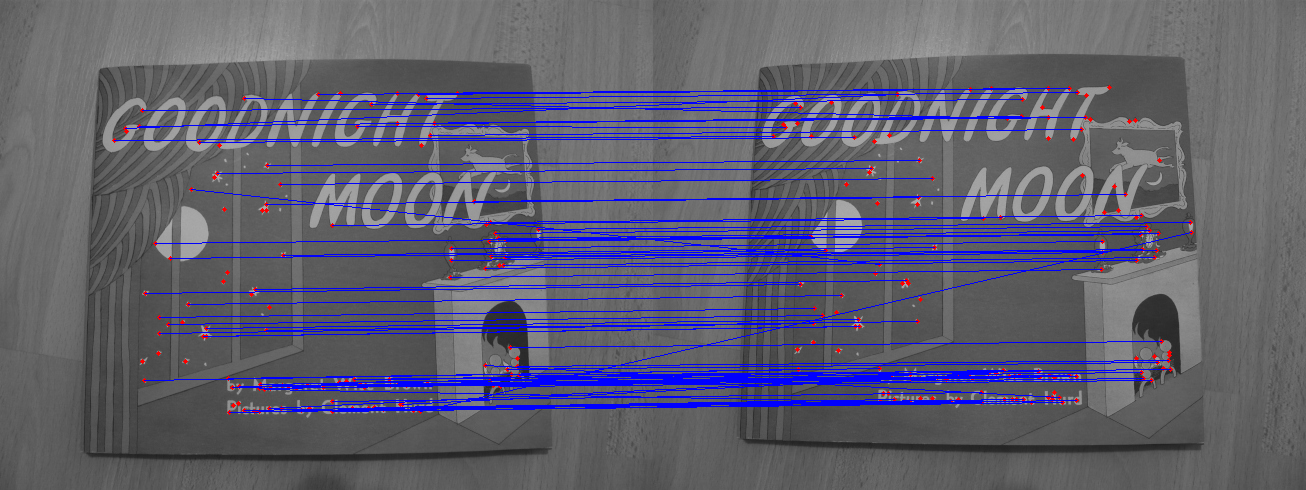
\includegraphics[width=\textwidth]{match_mutual.png}
%    \centering
%    \caption{Matching keypoints for mutual nearest neighbor matching}
%    \label{match_mutual}
%\end{figure}

\end{document}
